% =============================================================================
% CAPÍTULO 7 — volta 3 (AGENTS.md §6): a geometria do condicionamento.
%
% O fracasso que o abre, com número na mão: a taxa de rompimento deixa 34 de 36 explicações
% caberem nos mesmos dados — e o pior bloco de 60 dias não deixa nenhuma, porque a família de
% duas leis sem memória só alcança 11 contra os 20 do dado.
%
% Medição: lab/experimentos/E07_condicionamento.ipynb. Figuras: figuras/E07_condicionamento_*.
% =============================================================================

\chapter{Quantas explicações cabem}
\label{cap:condicionamento}

\section{A pergunta que o capítulo anterior deixou}

O capítulo anterior terminou reconhecendo que a conta dele estava contaminada: o corte é erguido
numa janela e o alvo é contado em janelas que se sobrepõem a ela. Tirar a sobreposição não é só
cautela de método; é reconhecer que um pedaço finito de passado carrega uma quantidade finita de
informação, e que essa quantidade pode não dar para tudo o que se quer perguntar.

Este capítulo mede essa quantidade com uma conta grosseira e direta. Toma-se uma família de
explicações --- todas as séries que se pode gerar com duas leis, uma calma e uma agitada ---, e
pergunta-se quantos membros da família reproduzem o que o dado mostra. A resposta tem duas
formas, e confundi-las é o erro que o capítulo persegue:

\begin{itemize}[leftmargin=1.5em]
  \item a estatística deixa uma \textbf{região}: muitas explicações cabem, e o dado não escolhe
    entre elas;
  \item a estatística corta o conjunto \textbf{a zero}: nenhuma explicação cabe, e o dado
    refutou a família inteira.
\end{itemize}

As duas são informação. A primeira diz o que ainda não se sabe; a segunda diz que a família
estava errada. Uma média entre as duas não diz nada.

\section{A família mais simples que existe}

A família tem dois parâmetros. O primeiro é \emph{p}, a fração de dias que passam no regime
agitado. O segundo é a razão entre as duas leis: quantas vezes o dia agitado é mais
agitado que o calmo. A oscilação global é mantida fixa em todos os membros, de modo que comparar
dois deles compare o mecanismo e não o tamanho.

O dado é a mesma série dos capítulos anteriores, com \numCondicionamentoDias{} dias, e as quatro
estatísticas que ele mostra: a taxa de rompimento de \numCondicionamentoTaxa, o pior bloco de
sessenta dias com \numCondicionamentoPior{} rompimentos, a mediana dos blocos em
\numCondicionamentoMediana, e a fração de blocos acima do dobro da promessa, que é de
\numCondicionamentoAcimaDoDobro. Um membro entra no conjunto quando as quatro cabem nas suas
tolerâncias: dois décimos de ponto percentual na taxa, dois rompimentos no pior bloco, um dia na
mediana e três centésimos naquela fração.

A primeira estatística é a do primeiro capítulo, e mede o nível. As outras três medem a forma com
que os rompimentos chegam, e é na forma que as explicações se separam.

\section{Com a taxa sozinha, quase tudo cabe}

A grade tem \numCondicionamentoCombinacoes{} membros. Exigindo apenas a taxa, dentro de uma
tolerância de dois décimos de ponto percentual, cabem \numCondicionamentoCabemTaxa{} deles.

Vale ler esse número devagar. \numCondicionamentoCabemTaxa{} explicações diferentes --- com frações agitadas
distintas e razões distintas entre as leis --- reproduzem o mesmo número que o primeiro capítulo discutiu. A promessa, sozinha, não identifica nada; ela é compatível com quase
toda a família. E isso não é defeito da família, é o que a estatística carrega: uma média não
guarda a forma.

\section{O pior bloco esvazia o conjunto}

Acrescentando o pior bloco de sessenta dias, o número que cabem passa a
\numCondicionamentoCabemTaxaPior{}.

O conjunto fica vazio, e não apenas pequeno. A família de duas leis, com
o estado sorteado de novo a cada dia, \textbf{não alcança} o agrupamento que o dado tem, e o teste é
direto: o melhor pior bloco que qualquer membro consegue produzir é de
\numCondicionamentoMelhorPior{} rompimentos, contra os \numCondicionamentoPior{} do dado.

Há uma coincidência que não é coincidência. Quando o primeiro capítulo submeteu duzentos mundos
que nunca mudam à mesma rotina, o pior bloco de todos eles parou em \numNuncaMudaPiorBloco. A família deste
capítulo chega perto desse teto sem alcançá-lo, e pelo mesmo motivo: sem memória, os dias ruins não têm como se
agrupar.

\begin{figure}[htbp]
  \centering
  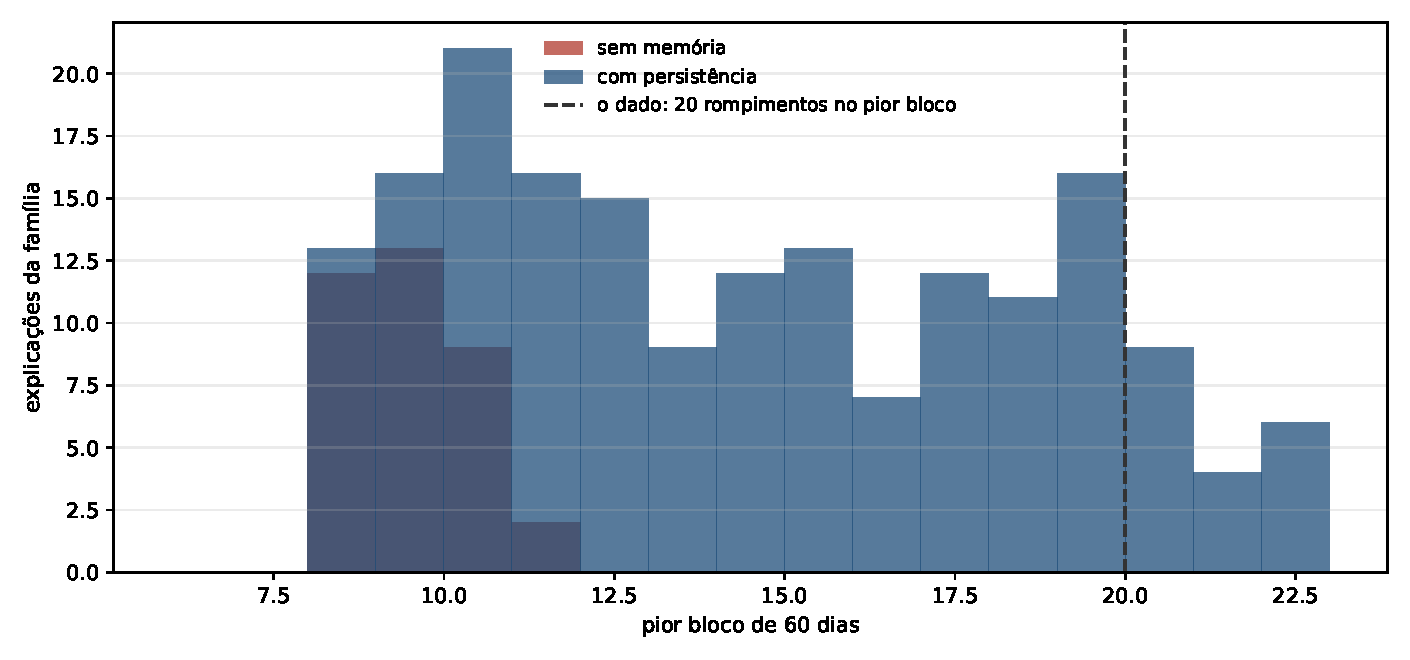
\includegraphics[width=\linewidth]{figuras/E07_condicionamento_1.pdf}
  \caption{Até onde cada família alcança o agrupamento do dado. A linha tracejada é o pior bloco
    que a série produziu; as barras são quantos membros de cada família chegam a cada valor. A linha colada na borda faz o vazio à esquerda parecer margem apertada; é um muro, e não uma folga.}
  \label{fig:alcance}
\end{figure}

\section{O estado que dura}

O que falta à família é a única coisa que o dado parece exigir: que o regime dure. Um terceiro
parâmetro entra, e ele é a permanência média do regime agitado, em dias. Com permanência de um
dia o dia agitado nunca é seguido de outro, e a família fica mais arrumada que a sem memória.

A grade passa a \numCondicionamentoPersistenteCombinacoes{} membros, e a resposta muda de
natureza. Com a taxa sozinha cabem \numCondicionamentoPersistenteCabemTaxa. Com a taxa e o pior
bloco, cabem \numCondicionamentoPersistenteCabemTaxaPior{}. Com as quatro estatísticas, cabem
\numCondicionamentoPersistenteCabemQuatro{} --- dois membros da família inteira, com permanências
curtas, da ordem de dez a trinta dias.

E o teto some: o melhor pior bloco que a família persistente alcança é de
\numCondicionamentoPersistenteMelhorPior{} rompimentos, que já cobre o que o dado mostra. O
excesso de blocos cheios também aparece, e até com folga: o maior valor da família é de
\numCondicionamentoPersistenteMelhorExcesso, contra \numCondicionamentoAcimaDoDobro{} do dado.

Uma explicação que reproduz as quatro estatísticas de uma série de \numCondicionamentoDias{} dias com dois
parâmetros e uma permanência é pouco. Duas explicações que as reproduzem são o resultado honesto
deste capítulo: o dado identifica uma \textbf{região}, e não um ponto.

\begin{figure}[htbp]
  \centering
  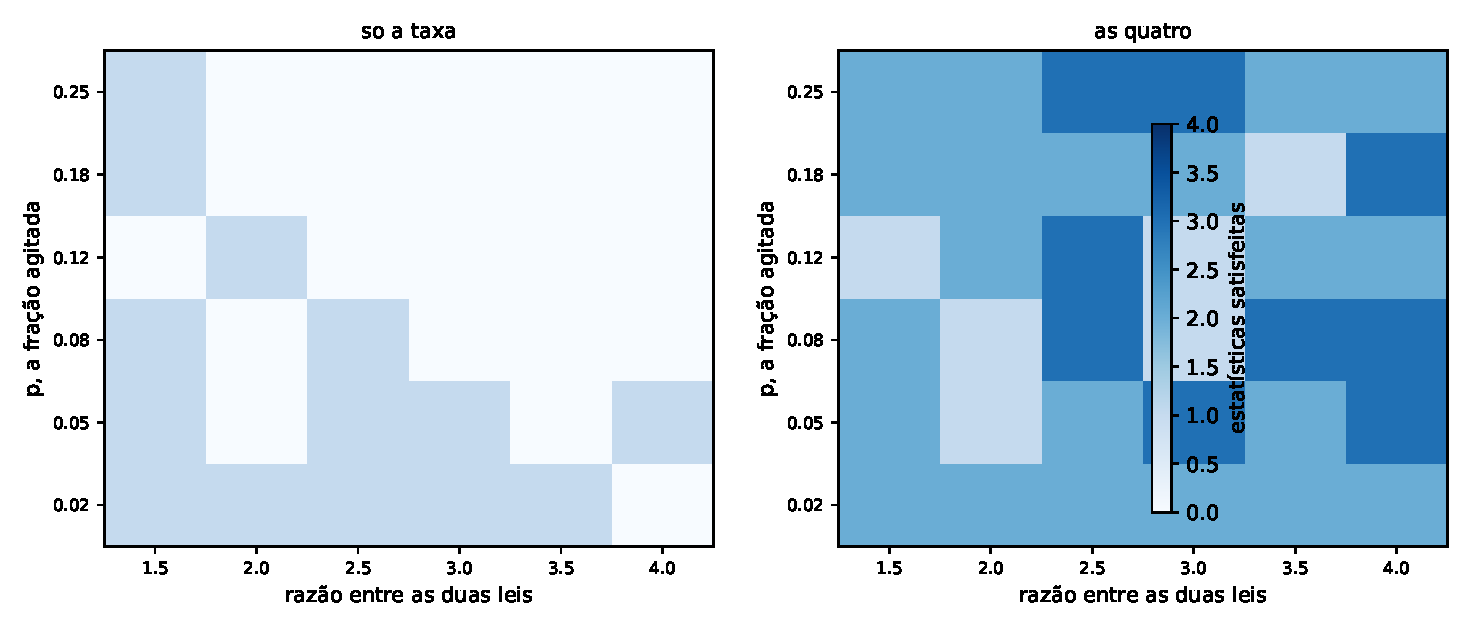
\includegraphics[width=\linewidth]{figuras/E07_condicionamento_2.pdf}
  \caption{O conjunto factível no plano dos dois primeiros parâmetros, para a permanência longa.
    À esquerda, os pontos que reproduzem a taxa; à direita, quantas das quatro
    estatísticas cada ponto satisfaz. A cor conta estatísticas satisfeitas, e não quão bom é o
    ajuste: escuro não é aprovação --- \numCondicionamentoPontosAsQuatro{} pontos da permanência
    mais longa chegam às quatro, e as \numCondicionamentoPontosSoATaxa{} da esquerda são as mais pálidas da escala.}
  \label{fig:factivel}
\end{figure}

O mapa da \cref{fig:factivel} diz o mesmo em duas dimensões. Na permanência mais longa,
\numCondicionamentoPontosSoATaxa{} dos \numCondicionamentoCombinacoes{} pontos do plano reproduzem a taxa, e \numCondicionamentoPontosAsQuatro{} reproduzem as quatro estatísticas --- o que confirma,
por outro caminho, que as duas explicações que sobrevivem têm permanência curta.

\section{O tamanho da região é de quem mede}

Falta o controle que separa o que é do dado do que é da minha escolha. A tolerância foi escolhida
por mim, e uma tolerância frouxa admite mais explicações por construção. E são quatro, uma por
estatística e na unidade da própria estatística: dois décimos de ponto percentual na taxa, dois
rompimentos no pior bloco, um dia na mediana e três centésimos na fração de blocos cheios. A conta foi repetida com
a tolerância apertada pela metade e com o dobro dela.

O veredito sobre a família sem memória não se move: \numCondicionamentoApertadaSemMemoriaTaxaPior{}
membros com a tolerância apertada, \numCondicionamentoEscolhidaSemMemoriaTaxaPior{} com a
escolhida e \numCondicionamentoFrouxaSemMemoriaTaxaPior{} com a frouxa. A refutação é do dado.

O tamanho do conjunto factível da família persistente, esse, depende da escolha:
\numCondicionamentoApertadaPersistenteQuatro{} explicações com a tolerância apertada,
\numCondicionamentoEscolhidaPersistenteQuatro{} com a escolhida e
\numCondicionamentoFrouxaPersistenteQuatro{} com a frouxa. Dizer "o dado identifica duas
explicações" sem dizer com que tolerância é dizer um número que pertence a quem mediu.

Vale a distinção, porque ela reaparece em tudo o que vem: \textbf{refutação é do dado; tamanho de
região é do critério}. O primeiro capítulo já tinha mostrado a versão disso numa estatística só
--- o corte assina a média ---, e aqui ela aparece na forma completa.

\section{O que fica}

Fica a \textbf{geometria}: uma família de explicações, um punhado de estatísticas, e o conjunto
dos membros que sobrevivem a todas. A taxa deixa uma região grande; o agrupamento dos dias ruins
corta essa mesma família a zero; a persistência a traz de volta, e as quatro estatísticas juntas
deixam duas explicações. Nenhuma delas é o ponto que uma medição sozinha promete.

E fica a disciplina que o capítulo repete de propósito: dizer "o modelo explica os dados" sem
dizer se o conjunto que sobra é uma região ou o vazio é uma frase sem conteúdo. Uma região
declarada é resultado; um vazio declarado é refutação; o resto é retórica.

O fracasso seguinte não está na conta, está no material. Encolher a região com mais estatísticas
tem limite, porque as quatro que usei são todas do mesmo pedaço de passado, do mesmo mercado. A
única coisa que ainda não tentamos é um mundo novo --- outro índice, outro período, outro
domínio ---, e a pergunta que fica é se ver mais mundos basta para escolher entre as duas
explicações que sobreviveram, ou se é preciso mexer no mundo de propósito para isso. É o que vem.
